
\section{Relativité restreinte}
\subsection{Électromagnétisme et relativité galiléenne}
Force de Lorentz : {\bf F} $=$ q({\bf E} + {\bf u} $\land$ {\bf B})
\begin{center} \begin{tikzpicture}
\draw [->] (0,0) --++ (1.5,0) node [below] {$x$};
\draw [->] (0,0) --++ (0,1) node [left] {$y$};
\node at (0,0) [left]{O};
\node at (0.5,0.5) [right]{$\mathcal{R}$};

\draw [->, very thick] (5,1.3) --++ (1.5,0) node [below] {${\bf v}$};
\draw [->] (4,0.3) --++ (1.5,0) node [above] {$x'$};
\draw [->] (4,0.3) --++ (0,1) node [left] {$y'$};
\node at (4,0.3) [left]{O'};
\node at (4.5,0.8) [right]{$\mathcal{R'}$};
\end{tikzpicture} \end{center}
\begin{enumerate}
  \item Dans $\mathcal{R'}$, la vitesse de la charge est ${\bf u'} = {\bf u} - {\bf v}$. On a alors :

\hspace{1.5cm}
\begin{minipage}[c]{.45\linewidth}
\begin{center}
Dans $\mathcal{R}$
\end{center}
\[
\begin{array}{rcr}
{\bf F} & = & \text{q}({\bf E} + {\bf u} \land {\bf B}) \\
 & = & 
\end{array}
\]
\end{minipage}
\hfill
\begin{minipage}[c]{.45\linewidth}
\begin{center}
Dans $\mathcal{R}$'
\end{center}
\[
\begin{array}{rcl}
{\bf F'} & = & \text{q}({\bf E'} + {\bf u'} \land {\bf B'}) \\
 & = & \text{q}({\bf E'} + ({\bf u} - {\bf v})\land {\bf B'}) \\
 & = & \text{q}({\bf E'} + {\bf u}\land {\bf B'} - {\bf v}\land {\bf B'}
\end{array}
\]
\end{minipage}

  \item D'après le principe de relativité (les lois physiques sont les mêmes dans tout les référentiels galiléen), la relation fondamentale de la dynamique donne :

\hspace{1.5cm}
\begin{minipage}[c]{.45\linewidth}
\begin{center}
Dans $\mathcal{R}$
\end{center}
\[
\begin{array}{rcr}
{\bf F} & = & \text{m}{\bf a} \\
 & = & \text{m d}_t{\bf u}
\end{array}
\]
\end{minipage}
\hfill
\begin{minipage}[c]{.45\linewidth}
\begin{center}
Dans $\mathcal{R}$'
\end{center}
\[
\begin{array}{rcr}
{\bf F'} & = & \text{m}{\bf a'} \\
 & = & \text{d}_t{\bf u'} \\
 & = & \text{d}_t(${\bf u} - {\bf v}$) \\
 & = & \text{m d}_t{\bf u}
\end{array}
\]
Car {\bf v} est constant.
\end{minipage}
On a donc : {\bf F'} $=$ {\bf F}.

En égalant l'expression des forces de Lorentz obtenuent dans chacun des référentiels, on obtient :
\[
{\bf E'} + {\bf u'} \land {\bf B'} = {\bf E} + {\bf u} \land {\bf B}
\]
Dans le référentiel ou la charge est au repos, {\bf u'} est nul, on a donc :
\[
{\bf E'} = {\bf E} + {\bf u} \land {\bf B}
\]
${\bf u} \land {\bf B}$ est le champ électromoteur.
 \item {\bf Dans le référentiel du laboratoire :} Pour des raisons de symétrie, le champ électrique créé par le fil est dirigé suivant ${\bf \hat{r}}$ et ne dépend que de r :
\[
{\bf E} = E(r).{\bf \hat{r}}
\]
\begin{minipage}[c]{.45\linewidth}
\begin{center}
\vspace{0.3cm}
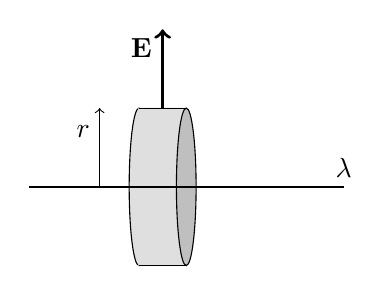
\begin{tikzpicture}
\filldraw [fill=gray!25,draw=black] (-0.6,0) ellipse (0.125cm and 1cm);
\filldraw [gray!25] (-0.6,-1) to [bend left=8] (-0.6,1) -- (0,1) to [bend right=8] (0,-1) -- cycle;
\filldraw [fill=gray!50,draw=black] (0,0) ellipse (0.125cm and 1cm);
\draw (-0.6,1) --++ (0.6,0);
\draw (-0.6,-1) --++ (0.6,0);
\draw [ <-, very thick] (-0.3,2) -- (-0.3,1) node [midway,above left] {\bf E};
\draw[thick] (-2,0)--(2,0);
\draw [ <-] (-1.1,1) -- (-1.1,0) node [midway,above left] {$r$};
\draw (2,0) node [above] {$\lambda$};
\end{tikzpicture}

\vspace{0.2cm}
Fig. 1: Surface de Gauss
\end{center}
\end{minipage}
\hfill
\begin{minipage}[c]{.45\linewidth}
 On applique le théorème de Gauss sur la surface grisée de la figure 1 : 
\[
\begin{array}{ c c c c }
 & \oint_{S}{\bf E}.{\bf dS} & = & Q / \epsilon_0 \\
\text{qui donne}  & E(r).2\pi r & = & \lambda / \epsilon_0 \\
\text{Soit}  & E(r)  &  = &  \frac{\lambda}{2\pi\epsilon_0 r} 
\end{array}
\]
\end{minipage}

\hspace{1.5cm}
{\bf Dans le référentiel en translation uniforme :}
Calculer les champs électrique et magnétique créés par le fil (à partir des équations de
Maxwell) d puis dans un 
à la vitesse v dans une direction parallèle au fil.
  \item Calculer l'expression de la force de Lorentz dans ces deux réferentiels et conclure.
\end{enumerate}

\subsection{Expérience de Michelson-Morley (1887)}

L'expérience de Michelson-Morley avait pour but de mettre en évidence la présence d'un hypothétique
éther dans lequel la Terre se déplace, et qui définit le référentiel d'inertie dans lequel la
lumière se propage à la vitesse c . Le résultat négatif de cette expérience est une des expériences
fondamentales qui ont mené à la relativité restreinte.
Le principe de l'expérience est de réaliser un interféromètre dit de Michelson (voir Fig. 2), qui
permet de comparer les temps d'aller-retour dans deux bras perpendiculaires de même longueur
L , lorsque ceux-ci sont en mouvement par rapport à l'éther. La longueur déployée des bras est de
L = 22 m . La source de lumière utilisée était une lampe à vapeur de Sodium de longueur d'onde
$\lambda$ = 589 nm . La Terre se déplace à v = 30 km.s −1 autour du Soleil.

\begin{center}
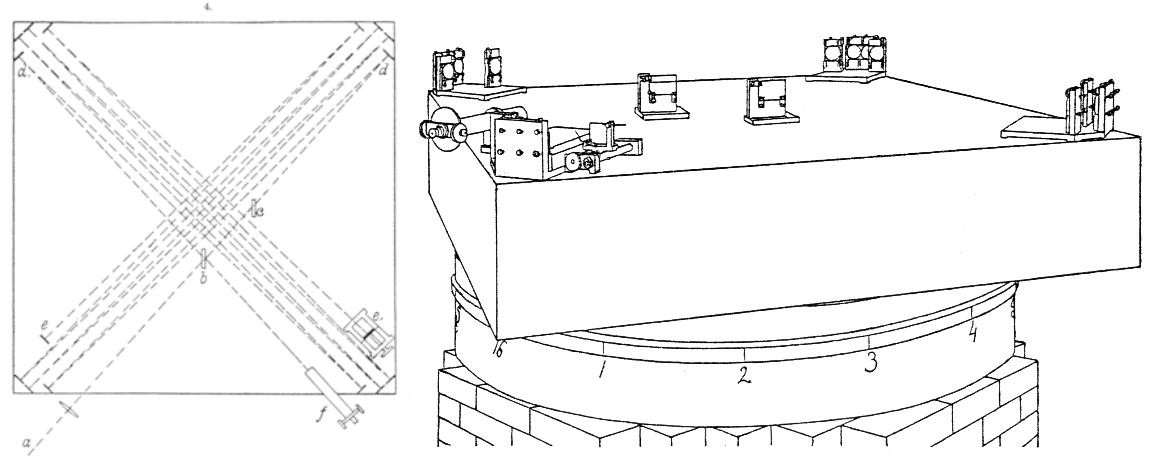
\includegraphics[scale=0.5]{./presentation/cropped-Michelson-morley-header}
%https://araz.community.uaf.edu/

Fig. 2: Principe et dispositif de l'expérience historique de Michelson-Morley.

{\it a : source lumineuse, b : lame semi-transparente, c : lame compensatrice, d : miroirs fixes, e : miroir réglable, f : occulaire}
\end{center}
\begin{enumerate}
  \item Effectuer un calcul de physique Galiléenne pour déterminer le temps d'aller retour d'un
flash lumineux le long de chacun des deux bras. On supposera que le mouvement de la
Terre coïncide avec la direction de l'un des bras.
  \item En déduire, dans la limite v ≪ c , le déphasage qui devrait être observé en sortie de l'interféromètre lorsqu'on éclaire l'interféromètre en lumière monochromatique. Comment observer
expérimentalement ce déphasage ?
  \item Le résultat de l'expérience historique a donné une absence de déphasage à mieux qu'un
centième de frange. Si l'éther existait, quelle serait sa vitesse maximale par rapport à la
Terre ? Commenter.
\end{enumerate}
\subsection{Désintégration de muons cosmiques}
Les muons sont des particules hargées ayant des propriétés très semblables aux éle trons excepté qu'ils sont plus massifs et instables. On les trouve en abondance dans les rayons cosmiques.
Leur durée de vie moyenne au repos a été mesurée et vaut : $\tau$ 0 = 2, 197 × 10 −6 s .
Un détecteur de muons est placé tout d'abord au sommet du Mont Washington (1910 m), puis
au pied de ette montagne, sensiblement au niveau de la mer. Dans sa première position, le
détecteur enregistre 563 +
− 10 muons par heure, dans sa seconde position, 408 +
− 9 .
\begin{enumerate}
  \item En faisant l'hypothèse que la vitesse des muons est proche de c , calculez leur durée de vie
moyenne $\tau$ telle qu'elle est mesurée par un expérimentateur terrestre.
En réalité, au cours de cette expérience, on a pu sélectionner des muons de vitesse v = 0, 992c .
  \item Montrez que l'expérimentateur peut retrouver cette valeur de $\tau$ à partir de la connaissance
de $\tau$ 0 .
\end{enumerate}
\subsection{Temps propre et temps impropre}
Une fusée quitte la Terre avec une vitesse $\beta$ ≡ v/c = 3/5 . Quand une horloge placée sur la
fusée indique qu'une heure s'est écoulée, la fusée envoie un signal lumineux à la Terre.
\begin{enumerate}
  \item Pour les horloges terrestres, quand le signal lumineux a-t-il été envoyé ?
  \item Pour les horloges terrestres, combien de temps après le départ de la fusée le signal a-t-il
atteint la Terre ?
  \item Pour les horloges de la fusée, combien de temps après le départ de la fusée le signal a-t-il
atteint la Terre ?
\end{enumerate}
\subsection{L'effet Doppler}
On considère une source ponctuelle S émettant des flashs lumineux sphériques à une fréquence
qui se propagent à la vitesse de la lumière c . Comme il est indiqué sur la Fig. 3, la source est
animée d'une vitesse v par rapport au référentiel du laboratoire, qui fait un angle $\theta$ avec l'axe
de visée (toujours dans le référentiel du laboratoire).
$\nu$ S '
S
v
q
r
O
Fig. 3 : Source S se déplaçant à la vitesse v par rapport à un observateur O fixe dans le référentiel
du laboratoire.
Un observateur immobile dans ce référentiel est placé au point O. On repère par le vecteur
r la position de la source qui a émis le signal présent en O. On suppose l'observateur éloigné,
c'est-à-dire r ≫ c/$\nu$ ' .
\subsubsection{Effet Doppler classique ( v ≪ c )}
\begin{enumerate}
  \item Dans le référentiel du laboratoire, exprimer la durée ∆t O séparant la réception de 2 flashs
pour l'observateur en fonction de ∆t S , période d'émission du signal dans le référentiel de
l'observateur.
  \item Interpréter graphiquement l'effet Doppler classique en représentant les crêtes correspondant
à 4 périodes successives sur un dessin. Y-a-t-il un effet Doppler classique transverse (pour
$\theta$ = $\pi$/2 ) ?
\setcounter{numero}{\theenumi}\end{enumerate}
\subsubsection{Effet Doppler relativiste}
\begin{enumerate}
  \setcounter{enumi}{\thenumero}
  \item Définir ensuite un référentiel dans lequel l'intervalle de temps séparant 2 flashs est un temps
propre et en déduire la fréquence $\nu$ O mesurée par l'observateur en fonction de v , $\theta$ et de la
fréquence $\nu$ S ' de la source.
\end{enumerate} 
\subsection{Diverses mesures de longueurs}
On considère une fusée voyageant à la vitesse v entre 2 planètes A et B séparées d'une distance L .
\begin{enumerate}
  \item Calculez l'intervalle de temps mesuré par une horloge de la fusée entre les 2 franchissements
de planètes.
  \item Déduisez en la longueur L ' mesurée par le pilote de la fusée entre les 2 planètes.
\setcounter{numero}{\theenumi}\end{enumerate}
On considère un appareil comportant une source d'éclairs E placée à égale distance de 2 miroirs
situés en A et B , eux-mêmes séparés d'une distance L (mesurée au repos). Comme il est indiqué
sur la figure 4, l'ensemble se déplace à une vitesse v par rapport au laboratoire.

La source émet un éclair au temps t = t ' = 0 juste quand elle passe devant le point E ' du
laboratoire. L'éclair atteint les points A et B , est réfléchi vers le laboratoire et laisse 2 marques
en A ' et B ' .
\begin{enumerate}
  \setcounter{enumi}{\thenumero}
  \item Trouvez les temps indiqués par des horloges situées en A , B , A ' et B ' quand l'éclair y arrive.
  \item Les événements : l'éclair est en A ' et l'éclair est en B ' sont-ils simultanés ?
\end{enumerate} 
Fig. 4 : Dispositif émettant un éclair en E et le réfléchissant en A et B .
